\section{Unsupervised Learning}

\subsection{Introduction}

\textbf{Supervised learning} --- classes are known and need a ``definition'', in terms of data. Methods are known as: classification, discriminant analysis, class prediction, supervised pattern recognition. \\

\textbf{Unsupervised learning} -- classes are initially unknown and need to be ``discovered'' with their definitions from the data. Methods are known as: cluster analysis, class discovery, unsupervised pattern recognition.

\subsection{Clustering}

Finding groups of items that are similar. Success of clustering if often measured subjectively. A dataset for clustering is just like a dataset for classification, but without the class! \\

Clustering algorithms form two broad categories: hierarchical methods and partitioning methods. \\

Hierarchical algorithms are either agglomerative (bottom-up) or divisive (top-down). In practice, hierarchical agglomerative methods are often used - efficient exact algorithms available. \\

Partitioning methods usually require specification of the number of clusters, then try to construct the clusters and fit objects to them. \\

Let \(X = \{e_1, \dots, e_n\}\) be a set of elements i.e. instances. Let \(\mathcal{C} = (C_1, \dots, C_l)\) be a partition of \(X\) into subsets. Each subset is called a cluster and \(\mathcal{C}\) is called a clustering. \\

Input data can have two forms
\begin{itemize}
    \item each element is associated with a real-valued vector of \(p\) features e.g. measurement levels for different features
    \item pairwise similarity data between elements, e.g. correlation, distance (dissimilarity)
\end{itemize}

The goal of clustering is to find a partition of \(X\) elements into homogenous and well-separated clusters. Elements from the same cluster should have high similarity.

\subsubsection{\(k\)-means Clustering}

Algorithm to cluster numerical data around \(k\) centroids i.e., means. Need to choose value for \(k\), and initialise the centroids. \\

Find a ``good'' clustering by iteratively assigning each data point to the nearest of the \(k\) centroids, then updating each centroid to reflect any points that have been re-assigned. \\

\(P(i)\) is the cluster assigned to the element \(i, c(j)\) is the centroid of cluster \(j\). \(d(v_1, v_2)\) the Euclidean distance between feature vectors \(v_1, v_2\). The goal is to find a partition \(P\) for which the error (distance) function \(E_P = \sum_{i = 1}^n d(i, c(P(i)))\) is minimum. Centroid is the mean or weighted average of points in the cluster.

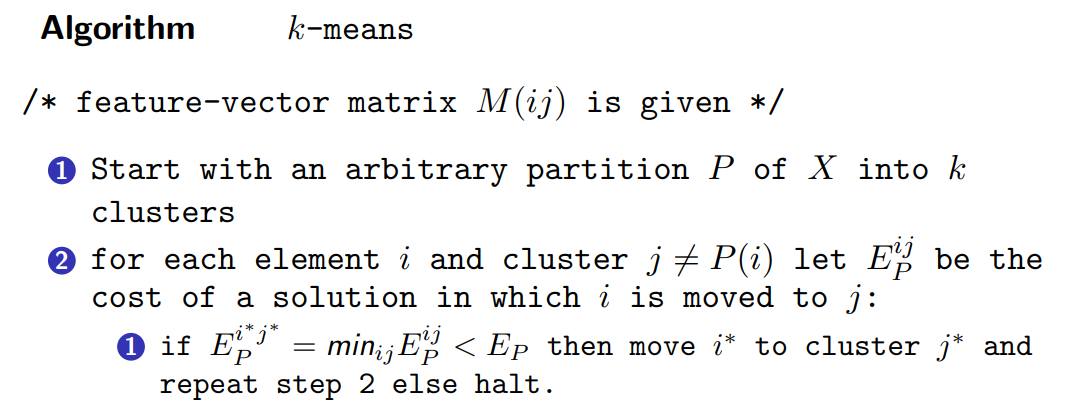
\includegraphics[scale=0.6]{assets/k_means.png}

\subsection{Hierarchical Clustering}

\begin{itemize}
    \item Bottom up: at each step join the two closest clusters (starting with single-instance clusters). Design decision: distance between clusters.
    \item Top down: find two clusters and then proceed recursively for the two subsets. Can be very fast.
    \item Both methods produce a dendrogram (tree of ``clusters'').
\end{itemize}

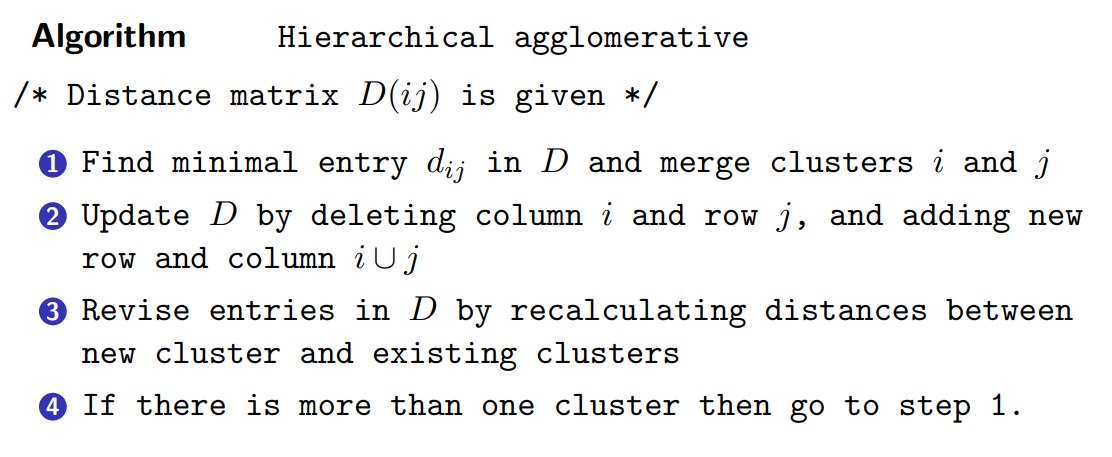
\includegraphics[scale=0.6]{assets/hierarchical_clustering.png}

\textbf{Dendrograms}. Two things to beware of:
\begin{enumerate}
    \item tree structure is not unique for given clustering - for each bottom-up merge the sub-tree to the right or left must be specified - \(2^{n - 1}\) ways to permute the \(n\) leaves in a dendrogram.
    \item hierarchical clustering imposes a bias - the clustering forms a dendrogram despite the possible lack of a implicit hierarchical structuring in the data
\end{enumerate}

\subsubsection{DBSCAN}

Density-based spatial clustering of applications with noise (DBSCAN). Defines clusters as dense regions of data instances. Density is based on having more than a minimum number of points (MinPts) within a radius \(\epsilon\). Does not force all points in the dataset to be members of clusters.

\begin{itemize}
    \item a core point has more than MinPts neighbours within \(\epsilon\)
    \item a border point has fewer neighbours than MinPts within \(\epsilon\), but is within \(\epsilon\) of a core point
    \item all other points are noise points
\end{itemize}

First, label all points as core, border or noise
\begin{itemize}
    \item Make a cluster for each core point, or set of connected core points. Core points are connected if they are within \(\epsilon\) of each other.
    \item assign each border point to the cluster of the corresponding core point
\end{itemize}

\subsection{Principal Component Analysis}

Performs a dimensionality reduction, finding a set of new features which preserves information in the original set.

This algorithm can be presented in several ways:
\begin{itemize}
    \item eigen-decomposition
    \item Singular Value Decomposition (SVD)
\end{itemize}

Can think of PCA as an SVD of the (mean-centred) matrix product \(\mathbf{X}^\top \mathbf{X}\). \\

PCA typically computed using the SVD and complexity is cubic in number of original features. This is not feasible for high-dimensional datasets.